% main.tex
\documentclass[12pt]{lab_thesis}
% プリアンブル
\usepackage{./preambles/jtygm}%%%%%%%%%%%%%%%%%Font Warning対策%%%%%
\usepackage[dvipdfmx]{graphicx}
\usepackage{bmpsize}
\usepackage{here}
\usepackage{comment}
\usepackage{amsmath, amssymb, amsthm, physics}
\usepackage{mathtools}% あからさまに読み込む
\usepackage{booktabs}
\usepackage[dvipdfmx,colorlinks=false]{hyperref}
\usepackage{pxjahyper}
\usepackage{titlesec}
\usepackage{wrapfig}
\usepackage{enumerate}
\usepackage{caption}
\usepackage{breqn}%数式dmath環境の使用
\usepackage{./preambles/listings, ./preambles/jlisting, color}% ソースコード関連
\usepackage{cleveref}
\usepackage[%
	backend=biber,
	style=numeric,
	sorting=none
]{biblatex}
\ExecuteBibliographyOptions{
  	sortcites=true,%\cite{}の中に書いた順番通りの出力する(falseなら並び替えない)
  	date=year,%dateの表示はyearのみにする
  	urldate=iso,%urldateの表示はyyyy-mm-ddにする
  	maxnames=8,%著者がmaxnamesを超えるときminnamesの数まで省略する
  	minnames=3,
  	%maxbibnames=99,%参考文献では99人まで著者を載せる
  	%backref=true,%引用したページを文献リストに表示する
  	%backrefstyle=none,%ページが連続するときの省略(デフォルトでthree)。省略させたくないときはnoneにする
	abbreviate=true,
  	isbn=false,%isbnを出力しない
  	url=false,
  	doi=true,
	arxiv=abs,
  	eprint=true,
	backref=true
}
% 参考文献ファイルの読み込み
\addbibresource{./references/reference_1.bib}

\crefformat{chapter}{第#2#1#3章}
\crefformat{section}{#2#1#3節}
\crefformat{subsection}{#2#1#3節}
\crefformat{enumi}{#2(#1)#3}
\crefrangeformat{enumi}{#3(#1)#4--#5(#2)#6}
\crefmultiformat{enumi}{#2(#1)#3}{,#2(#1)#3}{,#2(#1)#3}{,#2(#1)#3}

\numberwithin{equation}{section}
\crefname{equation}{式}{式}% {環境名}{単数形}{複数形} \crefで引くときの表示
\crefname{dmath}{式}{式}% {環境名}{単数形}{複数形} \crefで引くときの表示
\crefname{figure}{Fig.}{Fig.}% {環境名}{単数形}{複数形} \crefで引くときの表示
\crefname{table}{Tab.}{Tab.}% {環境名}{単数形}{複数形} \crefで引くときの表示

\newcommand{\crefpairconjunction}{と}
\newcommand{\crefrangeconjunction}{から}
\newcommand{\crefmiddleconjunction}{,}
\newcommand{\creflastconjunction}{,および}

% 図のキャプションのカスタマイズ
% https://karat5i.blogspot.com/2014/10/latex.html
\captionsetup[figure]{format=plain, labelformat=simple, labelsep=space, font=footnotesize}
% 「図」の表示名を変更
\renewcommand{\figurename}{Fig.}
\renewcommand{\tablename}{Table.}
% 図,表番号を"<章番号>.<図番号>” ,"<章番号>.<表番号>” へ
\renewcommand{\thefigure}{\thechapter.\arabic{figure}}
\renewcommand{\thetable}{\thechapter.\arabic{table}}
%数式フラグ:「eq:」
%図フラグ:「fig:」
% Christoffel記号
\newcommand{\chr}[3]{\Gamma^{#1}_{#2 #3}}
% クロネッカーのデルタ
\newcommand{\chron}[2]{\delta^{#1}_{#2}}
%Riemannテンソル
\newcommand{\Riemanntensor}[5]{
  \partial_{#3}\Gamma^{#1}_{#2 #4} - \partial_{#4}\Gamma^{#1}_{#2 #3} + \Gamma^{#1}_{#3 #5}\Gamma^{#5}_{#2 #4} - \Gamma^{#1}_{#4 #5}\Gamma^{#5}_{#2 #3}
}


% 論文情報の設定
\Title{サンプル論文タイトル}
\Author{山田 太郎}
\Professor{馬塲 一晴}
\StudentNumber{123456789}
% 卒業もしくは修了年度の設定
\Date{6}

% 論文種別の設定
%\master %修士論文の場合はこのコメントを外す
%\doctor %博士論文の場合はこのコメントを外す

\begin{document}
    % 表紙の作成
    \Maketitle

    % ページ番号をローマ数字に変更
    \pagenumbering{roman}
    % 目次の挿入
    \tableofcontents
    \clearpage
    % ページ番号をアラビア数字に戻す
    \pagenumbering{arabic}

    % 本文の開始
    \chapter{序 論}
卒業論文・修士論文は,みなさんのこれまでの研究の成果をまとめて報告し,みなさんがそれぞれの学位に値するかを審査するための重要な論文です.そのためには,これまでの研究成果の内容をよく吟味し,「人に自分の考えを伝える」重要性と難しさに注意し,分かりやすい表現を考え,書いた文章をよく推敲し,さらに,論文として定められた形式をとる必要があります.

    \chapter{\LaTeX の基本}
	\section{参考文献の引用方法}
	参考文献を論文中で引用するときはref.bibファイルに参考文献情報を貼り付けたうえで次のように引用しましょう\cite{G_ng_r_2021}.
	\section{数式について}
	文中式は $\hat{g}_{\mu\nu}=e^{2\omega}g_{\mu\nu}$ と書けます.その他別行立ての数式は次のような数式環境を用いて入力します.

	よく使用する数式については,./preambles/numerical\_formulas.texに,newcommandでマクロを定義しておくと便利です.
		\begin{equation}
			R_{\mu\alpha\nu}^{\lambda}=\Riemanntensor{\lambda}{\mu}{\alpha}{\nu}{\sigma}\label{eq:Riemann_tensor}
		\end{equation}

	また,複数行にわたる数式変形をきれいに出力したいときは,dmath環境を用いると便利です.dmath環境では数式を自動で改行したり,等号の位置を自動で揃えてくれます.
		\begin{dmath}
			R_{rr} = \partial_{\lambda}\chr{\lambda}{r}{r}
			- \partial_{r}\chr{\lambda}{\lambda}{r}
			+ \chr{\lambda}{\lambda}{\ell}\chr{\ell}{r}{r}
			- \chr{\lambda}{r}{\ell}\chr{\ell}{\lambda}{r}
			= \qty{\partial_{t}\chr{t}{r}{r} - \partial_{r}\chr{t}{t}{r} + \chr{t}{t}{\ell}\chr{\ell}{r}{r} - \chr{t}{r}{\ell}\chr{\ell}{t}{r}}
			+ \qty{\partial_{\theta}\chr{\theta}{r}{r} - \partial_{r}\chr{\theta}{\theta}{r} + \chr{\theta}{\theta}{\ell}\chr{\ell}{r}{r} - \chr{\theta}{r}{\ell}\chr{\ell}{\theta}{r}}
			+ \qty{\partial_{\varphi}\chr{\varphi}{r}{r} - \partial_{r}\chr{\varphi}{\varphi}{r} + \chr{\varphi}{\varphi}{\ell}\chr{\ell}{r}{r} - \chr{\varphi}{r}{\ell}\chr{\ell}{\varphi}{r}} \nonumber \\
			= \qty{\partial_{t}\chr{t}{r}{r} - \chr{t}{r}{r}\chr{r}{t}{r}}
			+ \qty{- \partial_{r}\chr{\theta}{\theta}{r} + \chr{\theta}{\theta}{t}\chr{t}{r}{r} + \chr{\theta}{\theta}{r}\chr{r}{r}{r} - \chr{\theta}{r}{\theta}\chr{\theta}{\theta}{r}}
			+ \qty{- \partial_{r}\chr{\varphi}{\varphi}{r} + \chr{\varphi}{\varphi}{t}\chr{t}{r}{r} + \chr{\varphi}{\varphi}{r}\chr{r}{r}{r} - \chr{\varphi}{r}{\varphi}\chr{\varphi}{\varphi}{r}} \nonumber \\
			= \frac{\dot{a}^2+a\ddot a}{1-Kr^2} - \frac{a\dot a}{1-Kr^2}\frac{\dot a}{a} + \frac{1}{r^2} + \frac{\dot a}{a}\frac{a\dot a}{1-Kr^2} + \frac{1}{r}\frac{Kr}{1-Kr^2} + \frac{\dot a}{a}\frac{a\dot a}{1-Kr^2} + \frac{1}{r}\frac{Kr}{1-Kr^2} -\frac{1}{r^2} \nonumber \\
			= \frac{2\dot{a}^2+a\ddot a + 2K}{1-Kr^2}\label{eq:Ricci_tensor}
		\end{dmath}

	論文中の数式を引用したい場合は,引用したい数式にラベルを付け,引用したい箇所で「\textbackslash cref\{eq:作成したラベル\}」と入力すれば\cref{eq:Ricci_tensor}のように引用が可能です.数式ラベル内にeq:とつけているのは数式をエディタの検索機能や補完機能を利用しやすくするためです.

	その他,数式を入力する際には,physicsパッケージを用いるのが便利です(usepackageしてあります).

	\section{図の挿入と引用}
	図は以下のように挿入できます.
		\begin{figure}[htbp]
			\centering
			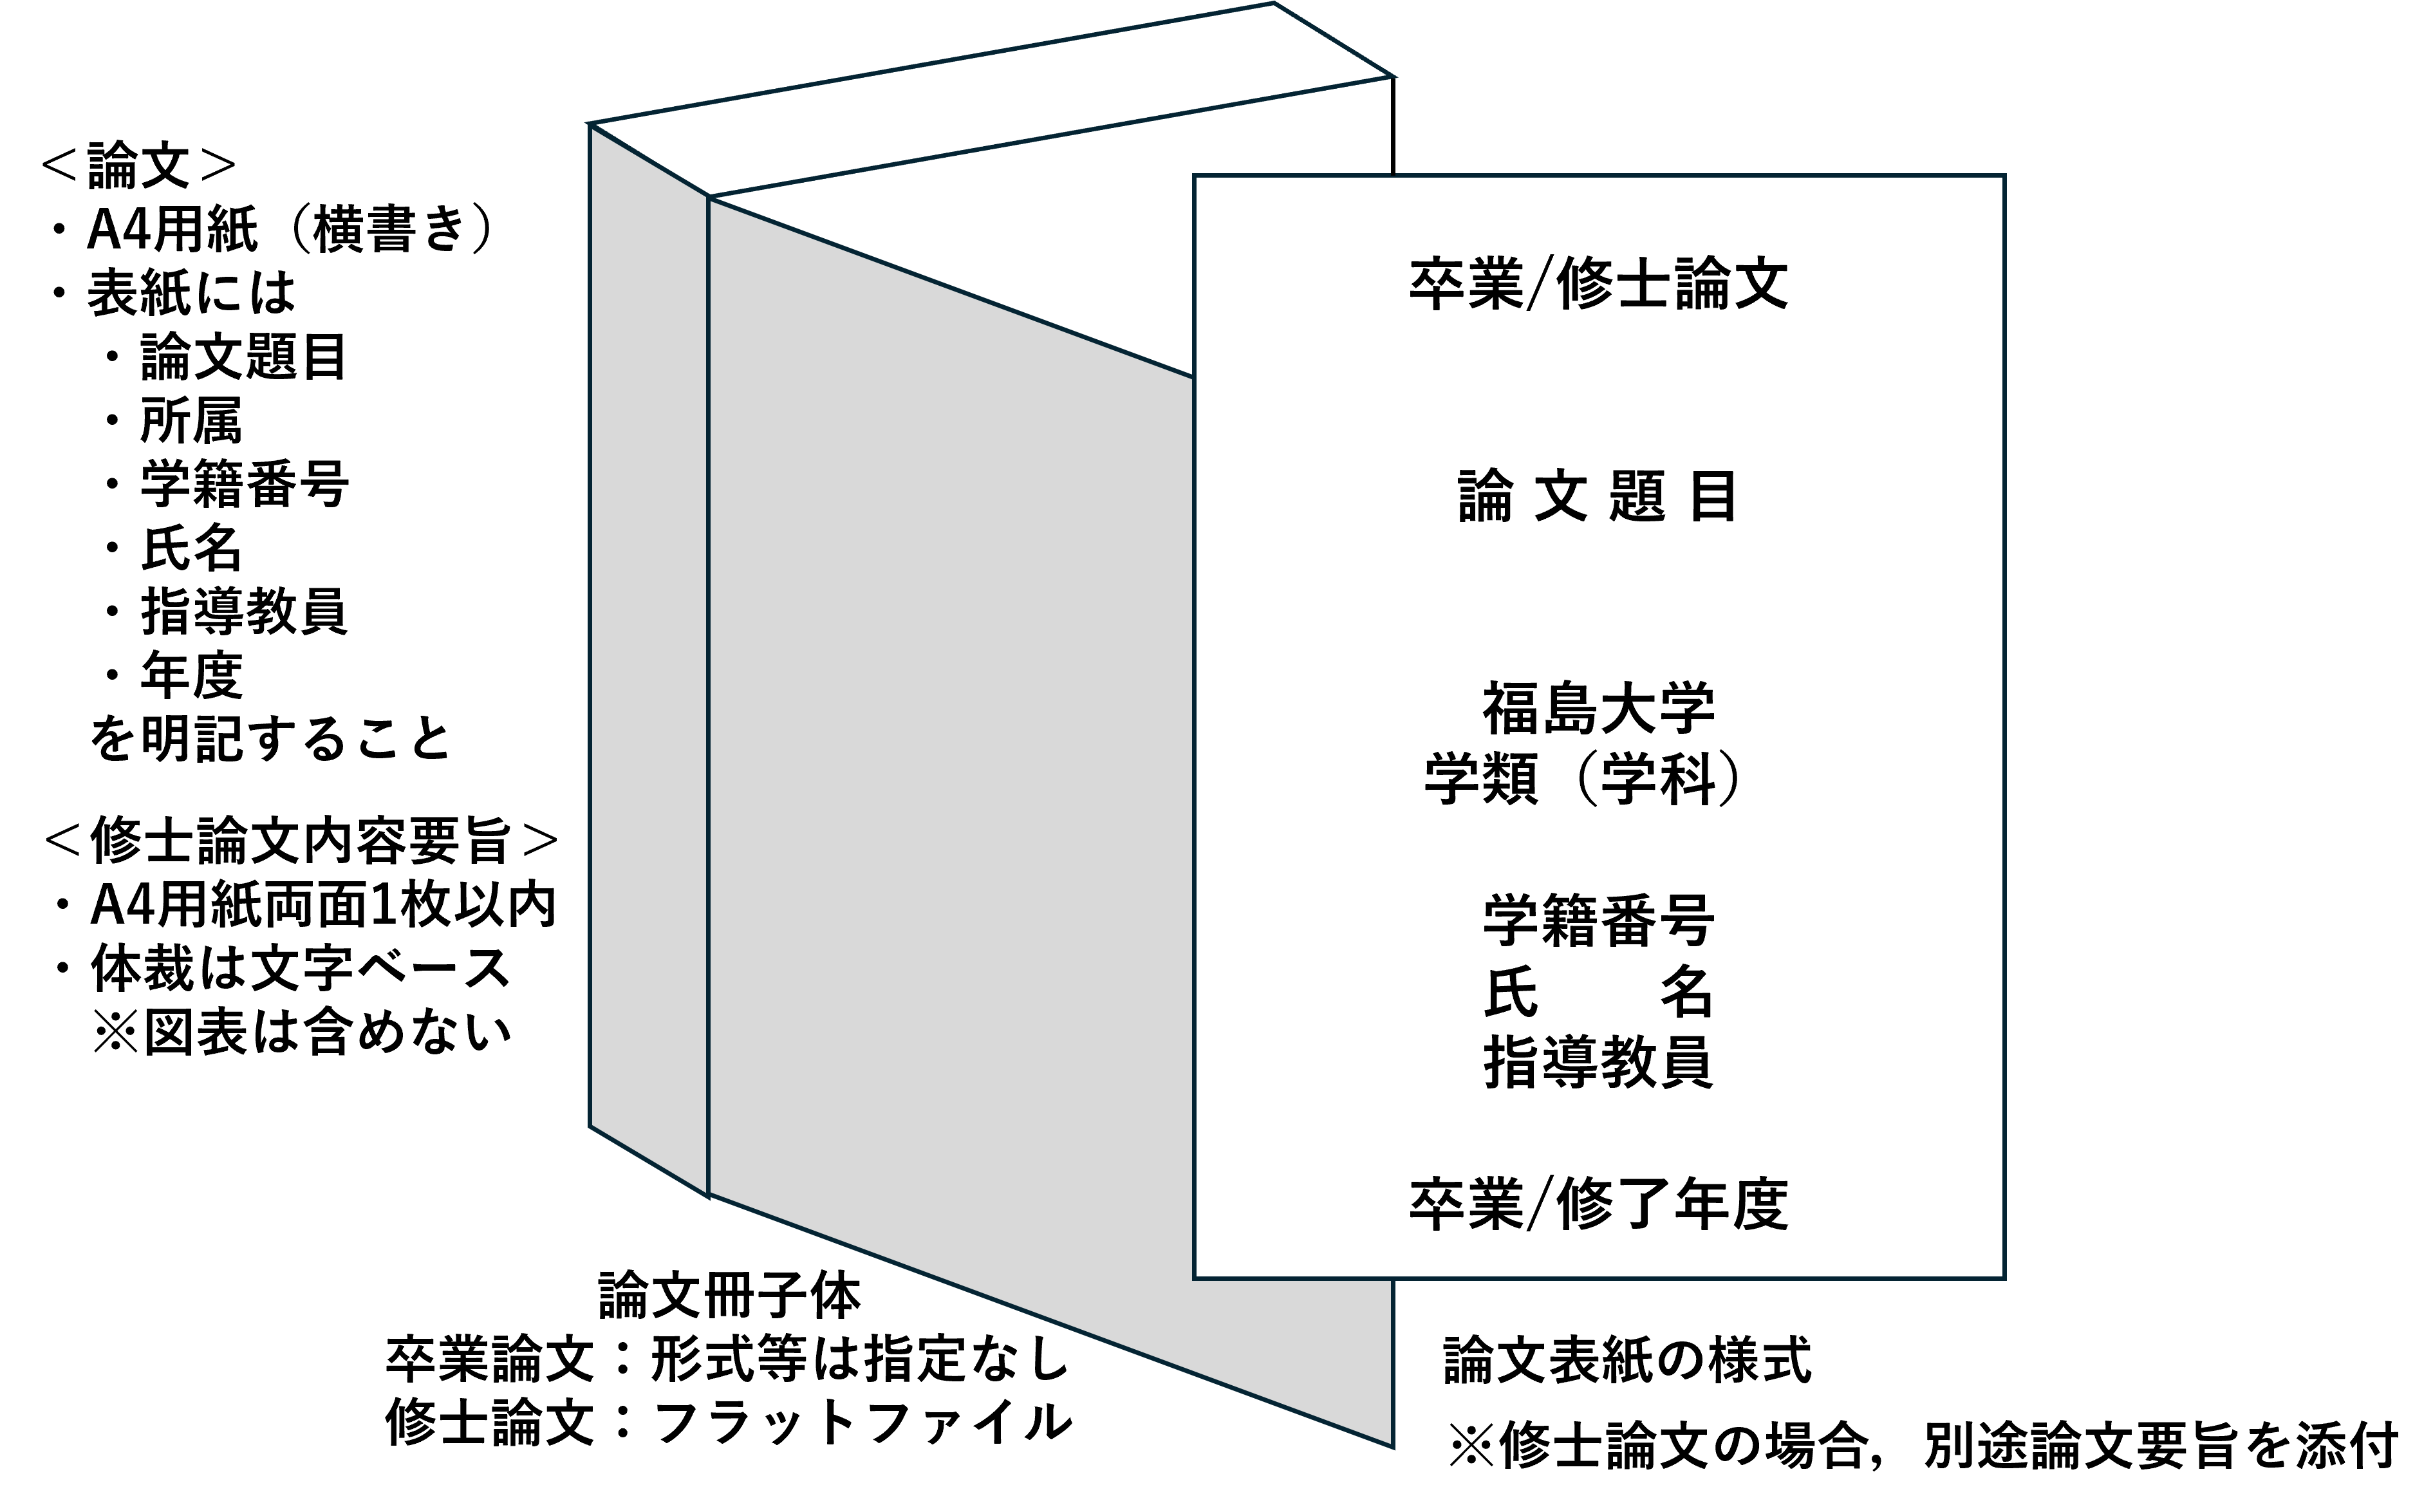
\includegraphics[width=1.0\linewidth,keepaspectratio]{./images/論文様式.png}
			\caption{論文の様式}
			\label{fig:overview}
		\end{figure}

	また,文中の図を引用したい場合は,図にラベルを付けて\cref{fig:overview}としましょう.

	\section{付録へのソースコードのつけ方}
	付録にソースコードをつける場合,本テンプレートに付属の「jlisting.sty」を以下の手順で適切な場所に置く必要があります.

		\begin{enumerate}
			\item jlisting.sty をC:\textbackslash texlive \textbackslash texmf-local\textbackslash tex \textbackslash latex\textbackslash local \textbackslash listings ディレクトリに置く(listingsディレクトリがなければ作成).
			\item 管理者モードのコマンドプロンプトで「mktexlsr」と入力し実行.
		\end{enumerate}

	これで問題なく実行できるはずです.


    \chapter{本 論 2}
    \section{結 果}
っこここっこkkkkkkkkkkkkkkkkkkkkkkkkkkkkkkkkkkkkkkkkkkkkkkkkkkkkkkkkkkkkkkkkkkkkkkkkkkkkkkkkkkkkkkkkkkkkkkkkkkkkkkkkkkkkkkkkkkkkkkkkkkkkkkkkkkkkkkkkkkkkkkkkkkkkkkkkkkkkkkkkkkkkkkkkkkkkkkkkkk

llllllllllllllllllllllllllllllllllllllllllloooooooooooooooooooooooおおおおおおおおおおおおおおおおおおおおおおおおおおおおおおおおおおおおおおおおおおおおおおおおおおおおおおおおおおおおおおおおおおおおおおおおおおおおおおおおおおおおおおおおおおおおおおおおおおおおおおおおおおおおおおおおおおおおおおおおおおおおおおおおおおおおおおおおおおおおおおおおおおおおおおおおおおおおおおおおおおおおおおおおおおおおおおおおおおおおおおおおおおおおおおおおおおおおおおおおおおおおおおおおおおおおおおおおおおおおおおおおおおおおおおおおおおおおおおおおおおおおおおおおおおおおおおおおおおおおおおおおおおおおおおお


もおおおおおおおおおおおおおおおおおおおおおおおおおおおおおおおおおおおおおおおおおおおおおおおおおおおおおおおおおおおおおおおおおおおおおおおおおおおおおおおおおおおおおおおおおおおおおおおおおおおおおおおおおおおおおおおおおおおおおおおおおおおおおおおおおおおおおおおおおおおおおおおおおおおおおおおおおおおおおおおおおおおおおおおおおおおおおおおおおおおおお

llllっぉおおおおおおおおおおおおおおおおおおおおおおおおおおおおおおおおおおおおおおおおぉおおおおおおおおおおおおおおおおおおおおおおおおおおおおおおおおおおおおおおおおおおおおおおおおおおおおおおおおおおおおおおおおおおおおおおおおおおおおおおおおおおおおおおおおおおおおお

    \chapter{結論}


    % 謝辞
    \thanks
    ここに謝辞をしたためます.
    \endthanks

    % 付録の開始
    \appendix
    \appendix
\appendixstyle
\chapter{数値解析コード}\label{appendix:code1}
ソースコード等を付録として示す場合は以下のようにしましょう.
%ソースコードのPathはmain.tex側から見た時のPathを指定
\lstinputlisting[caption = 使用した数値解析コード, label = lst:program2]{./source_codes/source_code_1.py}
\section{その他の付録}
付録における数式番号の出力スタイルのテストです.
\begin{equation}\label{eq:test_1}
    E=mc^2
\end{equation}

\cref{eq:test_1}は有名な式です(付録\ref{appendix:code1}).

付録ソースコード参照用独自マクロのテストです.\lref{lst:program2}はPythonのコードです.

付録参照用独自コマンドのテストです.\aref{appendix:code1}は数値解析コードです.

\chapter{huhuu}

    % 参考文献の出力
    \printbibliography[title=参考文献]

\end{document}
